\documentclass[a4paper,10pt]{report}
\usepackage[cm]{fullpage}
\usepackage[utf8]{inputenc}
\usepackage{amsmath}
\usepackage{amsthm}
\usepackage{amssymb}
\usepackage{appendix}
\usepackage{booktabs}
\usepackage[table]{xcolor}
\usepackage{amssymb}
\usepackage{multirow}
\usepackage{fullpage}
\usepackage{float}
\usepackage{wrapfig}
\usepackage{subfig}
\usepackage{graphicx}
\usepackage{listings}
\usepackage{color}
\usepackage{textcomp}

\usepackage{sagetex}

\usepackage{hyperref}

\definecolor{listinggray}{gray}{0.9}
%\definecolor{lbcolor}{rgb}{0.9,0.9,0.9}

\addtolength{\voffset}{-10pt}

\hypersetup{colorlinks=false}
 
\lstset{
%	backgroundcolor=\color{lbcolor},
	tabsize=4,
%	rulecolor=,
	language=python,
        basicstyle=\scriptsize,
        upquote=true,
        aboveskip={1.5\baselineskip},
        columns=fixed,
        showstringspaces=false,
        extendedchars=true,
        breaklines=true,
        prebreak = \raisebox{0ex}[0ex][0ex]{\ensuremath{\hookleftarrow}},
%        frame=single,
        showtabs=false,
        showspaces=false,
        showstringspaces=false,
        identifierstyle=\ttfamily,
        keywordstyle=\color[rgb]{0,0,1},
        commentstyle=\color[rgb]{0.133,0.545,0.133},
        stringstyle=\color[rgb]{0.627,0.126,0.941},
} \hypersetup{colorlinks=false}

\renewcommand\chaptername{Esperimento}
 
\DeclareGraphicsExtensions{.pdf,.png,.jpg}


\author{Marco Giglio, Maria Cristina Fortuna, Riccardo Iaconelli}
% Title Page
\title{Relazioni dal Laboratorio di Fisica 2}

\begin{document}

\maketitle

\tableofcontents

\chapter{Misura della velocità della luce}

L'obiettivo del nostro esperimento è misurare la velocità della luce $c$.

L'apparato di misurazione consiste principalmente in:
\begin{itemize}
 \item Un laser Elio-Neon ($\lambda=32$ nm).
 \item Uno specchio rotante a velocità angolare regolabile.
 \item Due lenti convergenti, di lunghezza focale $l_1 = 48mm$ e $l_2 = 252 mm$.
 \item Un microscopio con beam splitter e micrometro.
\end{itemize}

Lo specchio rotante viene fatto girare con velocità angolare $\omega_1$ in senso orario e $\omega_2$ in senso antiorario. Queste velocità angolari sono identiche nella maggior parte dei casi, e la loro differenza è trascurabile.

Chiamando $s_{cw}$ e $s_{ccw}$ rispettivamente le misure con specchio rotante in senso orario e antiorario, per come è orientata la strumentazione il numero
$$\Delta s = s_{cw} - s_{ccw}$$
deve essere positivo.

Purtroppo però non è questo il caso per qualche misura presa in mattinata, per ragioni sconosciute e che non siamo riusciti a riprodurre. Questi dati sono esclusi dalla misurazione in quanto evidenti errori, e sono mostrati in rosso nel grafico seguente
I dati sono molti, dunque forniamo qui soltanto una visione grafica, e lasciamo la tabella come allegato.

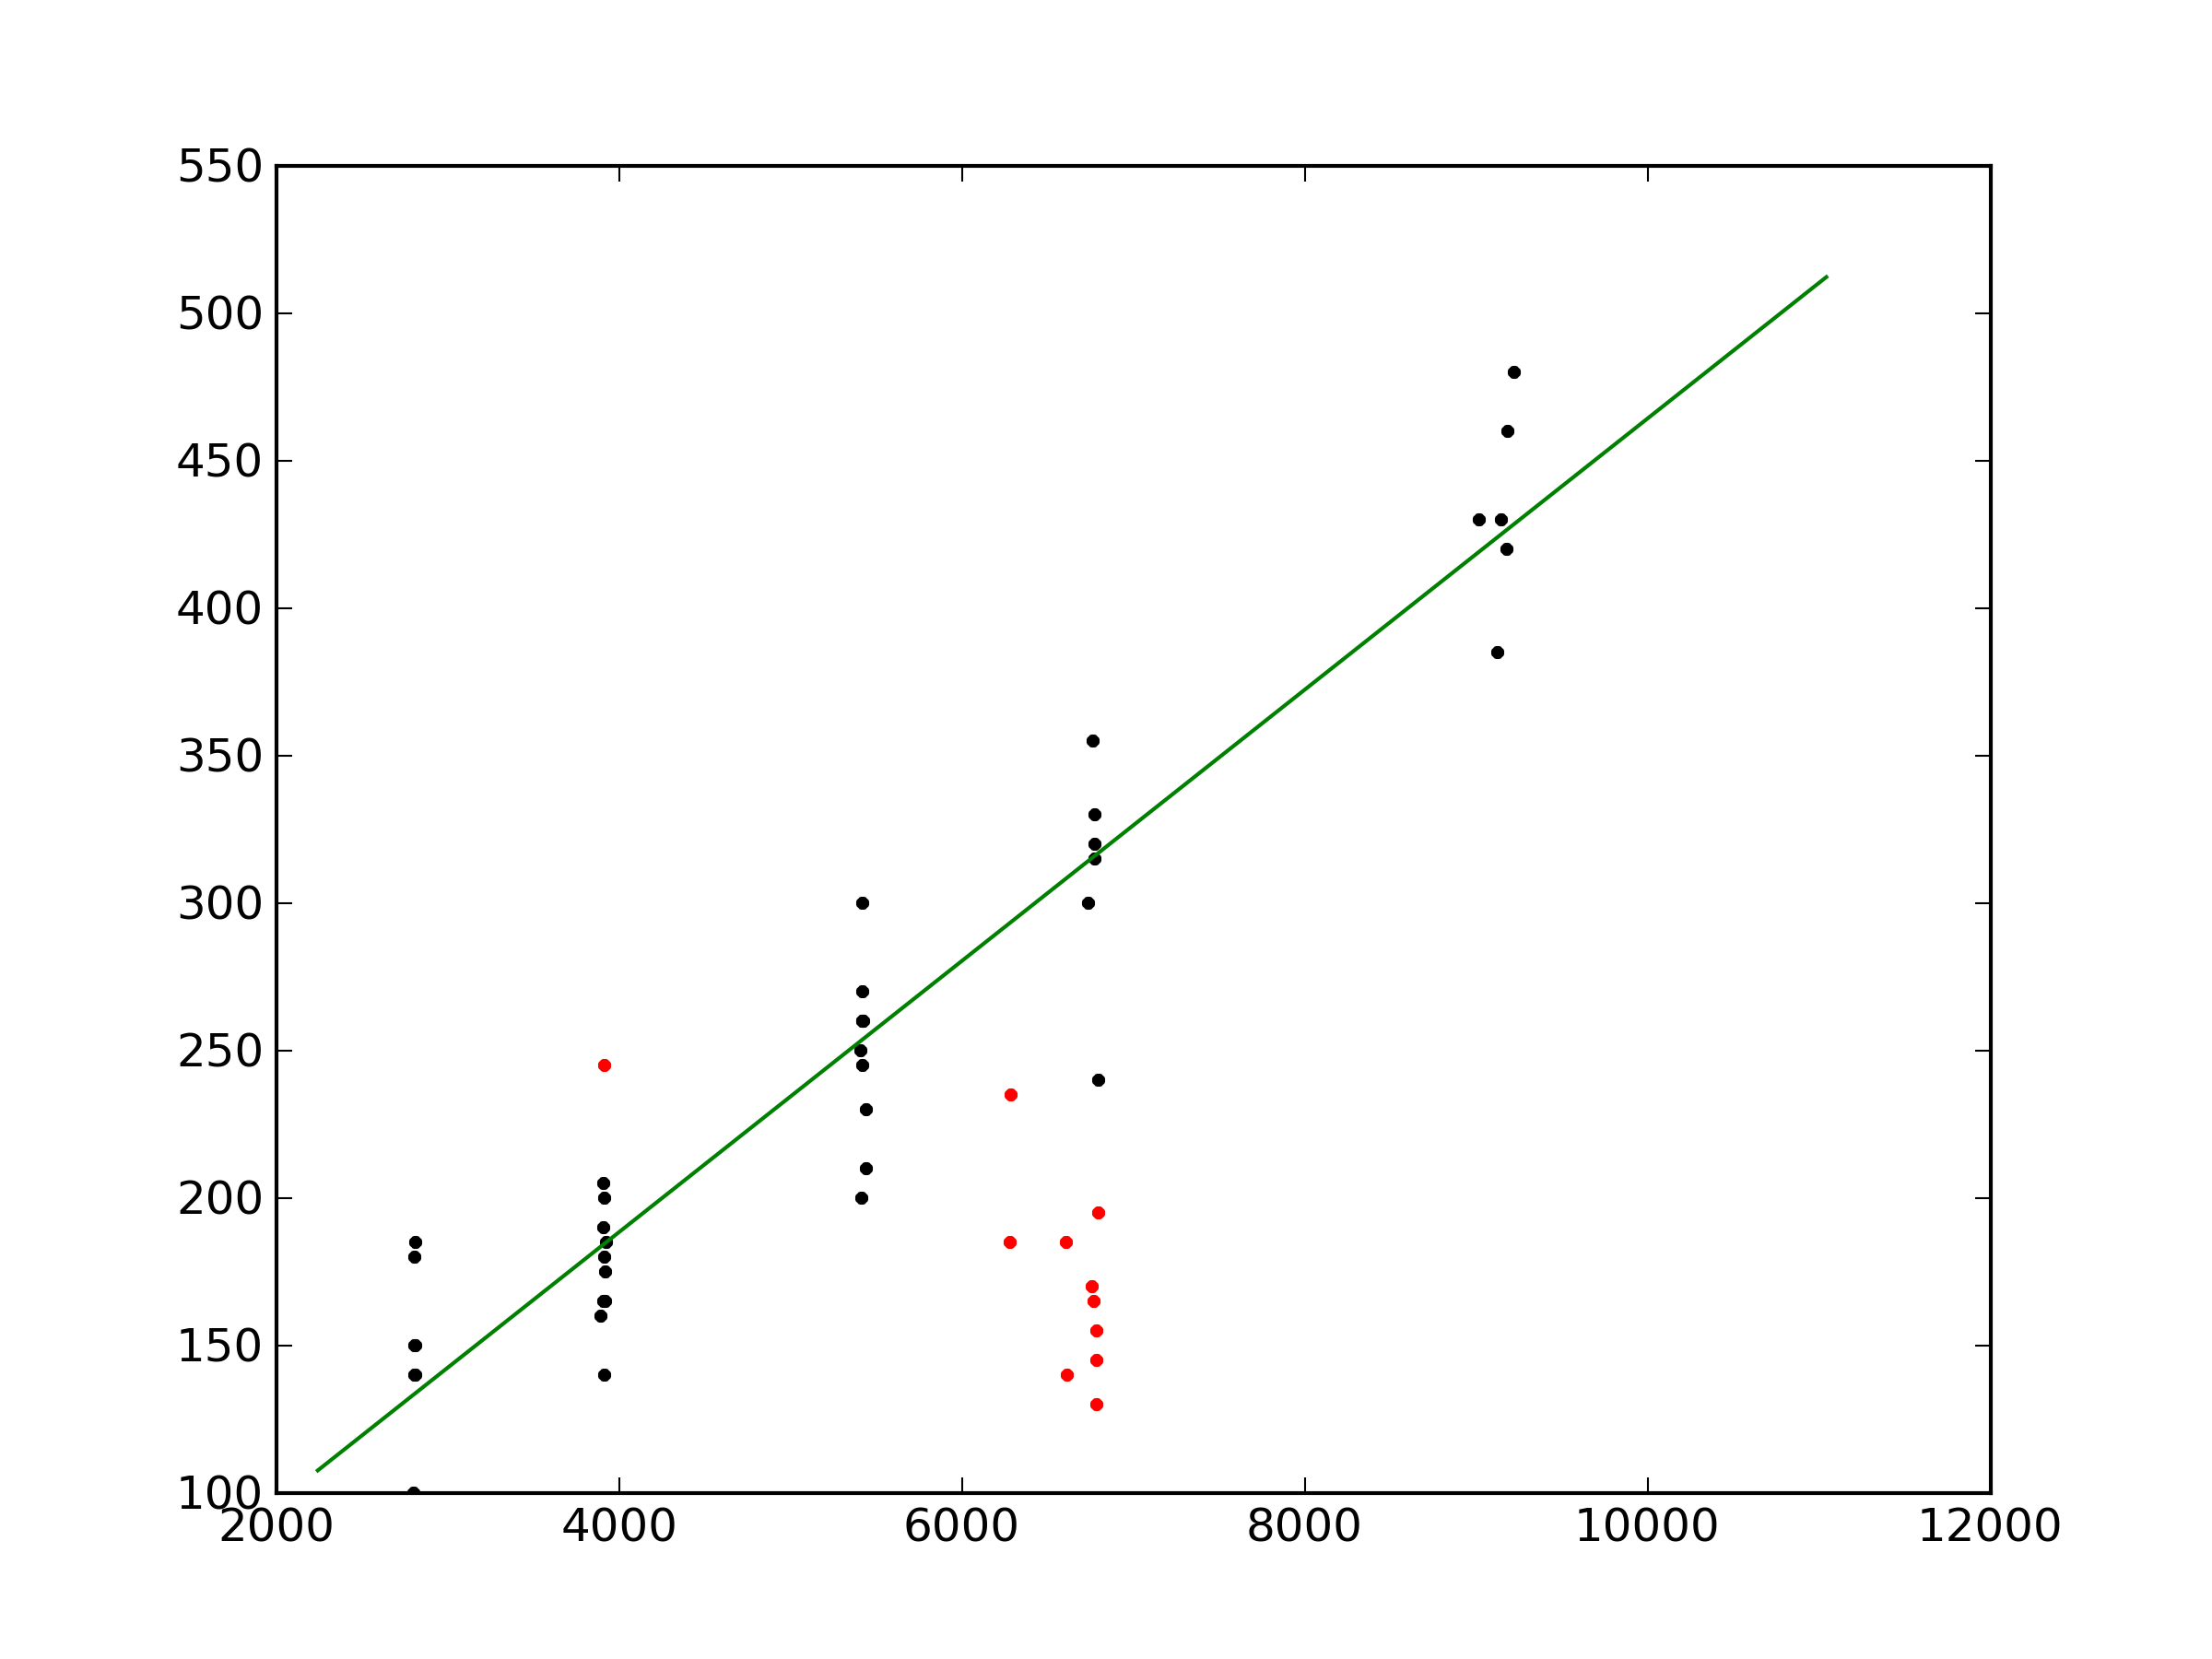
\includegraphics[scale=0.75]{grafici/C/dati.png}

\section{Analisi dati}

Chiamiamo $D = 13.480$m il cammino geometrico della luce per tornare allo specchio rotante, ovvero il doppio della distanza specchio rotante/specchio fisso; $A$ la distanza del punto di convergenza del fascio laser dalla lente $l_2$ e $B$ la distanza tra $l_2$ e lo specchio rotante. 

Per calcolare con precisione $A$, conoscendo la distanza focale di $l_2$, la ricaviamo dalla formula dei punti coniugati:
$$A=\frac{(B+D)f}{B+D-f} = 256\text{mm}$$


Per calcolare $c$, dobbiamo interpolare i dati presi nel modo seguente:
$$\Delta s = \frac{\tilde{A}}{c}\omega$$
ove
$$\tilde{A} = \frac{4*A*D^2}{2}$$

$\sage{2*e^2}$

La funzione che ci permetterà di calcolare $c$ è la seguente:

$$c = \frac{\tilde{A}}{m}$$
ove

Data una 
m=0.04594423946498933

Ricaviamo, tramite  il fit della funzione $V=R*I$" dove R è parametro da stimare, due resistenze ignote.


Misuro la resistenza interna del voltometro, mantenendo costante la ddp a $14.5\ V$ e variando la resistenza all'interno del circuito. 
Il voltmetro è in parallelo al circuito, perciò $R_i$:

$$R_i = \frac{RV}{RI-V} $$

dove R è la resistenza variabile, I la corrente nel circuito e $V= 14.5\ V$


La resistenza risulta $9.20 \pm 0.27 \ M \Omega$.


Misuriamo la resistenza interna dell'amperometro, che è collegato in serie al circuito. 

$$R_i = \frac{V-RI}{I}$$

In questo caso, R è fissato ($R=0.5 \Omega$) e sono V e I a variare

La resistenza interna risulta $11.42 \pm 0.45 \Omega$



Colleghiamo una piccola lampada a filamento al circuito, e verifichiamo che il suo comportamento resistivo non segue la legge di Ohm. 






\begin{sagesilent}
import numpy as np

rc = np.recfromcsv("dati/C2-RC.csv")
rl = np.recfromcsv("dati/C2-RL.csv")


def stampa_dati(wa, header):
  s = r"\begin{tabular}{c*{" + "%d" % (len(wa.dtype)-1)
  s += r"}{|c}}"
  s += "%s \\\\" % (header)
  s += r"\midrule"
  for i in range(0, len(wa)):
    a = ["%s" %x for x in wa[i]]
    s += "%s \\\\" % join(a, "&")
  s += r"\end{tabular}"
  return s
\end{sagesilent}



\chapter{C2}

\section{Risposta in frequenza del multimetro}



\begin{center}
\includegraphics[scale=0.75]{grafici/C2/cv.png} 
\end{center}

Per il grafico in alto,che mostra la lettura dell'intensità di corrente in funzione della frequenza, l'errore è dato dalla sensibilità dello strumento: $\sigma_i = 0.1\ mA$.
\

Il secondo grafico, che mostra i limiti operativi del multimetro rispetto la frequenza, L'errore sulla lettura dal multimetro è la sensibilità dello strumento: $\sigma_{mu} = 0.005\ V$. Per stimare l'errore su $V_{RM}$ abbiamo usato la deviazione standard, assumendo quindi che $V_{RMS}$ dovrebbe rimanere costante. 
Indi per cui, la propagazione degli errori risulta:
$$\sigma_r = \sqrt{\frac{\sigma_{mu}^2}{V_{RMS}^2} + \frac{\sigma_{rms}^2}{V_{RMS}^4}}$$

%E' giusto pensare che rimanga costante?f'

\section{Misura di impedenze ignote}

Scopo di questa seconda parte è misurare l'impedenza di un circuito RC e RL in frequenza alternata. Mostreremo la dipendenza di Z dalla frequenza.


\begin{center}

%\sagestr{stampa_dati(rc, r"Frequenza (Hz) & I (mA) & Valore mu & $V_{rms}$ (V)")}
\end{center}


\begin{center}
\includegraphics[scale=0.75]{grafici/C2/rc.png} 
\end{center}

Dal fit ricavo: $C = 374.53\pm8.44 nF$, che rientra nei valori aspettabili, dato che il valore teorico è $367 nF$. 
Il $chi^{\tilde}^2= 1.4461 $ 

%chi quadro rotto da sistemare.

\begin{center}

%\sagestr{stampa_dati(rl, r"Frequenza (Hz) & I (mA) & Valore mu & $V_{rms}$ (V)")}
\end{center}



\begin{center}
\includegraphics[scale=0.75]{grafici/C2/rl.png} 
\end{center}

$L = 0.016074\pm 0.000092 H$
$\chi^{\tilde}^2 = 1.4546$





%\chapter{Misura di resistenze}

L'obiettivo del nostro esperimento è misurare la validità della legge di Ohm per varie configurazioni di un circuito. 

Al fine di misurare corrente e potenziale, colleghiamo al nostro circuito due multimetri digitali. Il primo, che ha la funzione di voltmetro, lo poniamo ai capi della nostra resistenza collegato in parallelo; il secondo, in modalità amperometro, è posto in serie subito dopo la resistenza. 

Di seguito, gli strumenti con la loro precisione:
- Voltmetro (multimetro portatile), resistenza interna: 6 $M\Omega$
- Amperometro (multimetro da banco)
- Generatore da banco, resistenza interna ignota.


\section{Analisi dati}

Ricaviamo, tramite  il fit della funzione $V=R*I$" dove R è parametro da stimare, due resistenze ignote.

\subsection{Dati}

\begin{center}
\begin{tabular}{*{4}{c}}
Corrente1 & Potenziale1 & Corrente2 & Potenziale2\\
\midrule
396 & 201 & 3043 & 207\\
512 & 261 & 3667 & 250\\
706 & 360 & 4703 & 319\\
890 & 454 & 6365 & 432\\
1126 & 574 & 8984 & 609\\
1242 & 633 & 12326 & 836\\
1557 & 794 & 16898 & 1145\\
1812 & 925 & 340 & 24\\
1971 & 1005 & 725 & 50\\
2290 & 1168 & 966 & 66\\
2524 & 1286 & 1595 & 108\\
2850 & 1454 & 1822 & 124\\
3116 & 1589 & 2160 & 146\\
3407 & 1737 & 2302 & 157\\
3883 & 1980 & 2584 & 176\\
4229 & 2157 & 3100 & 211\\
4598 & 2344 & 3370 & 229\\
5072 & 2586 & 4036 & 274\\
5505 & 2807 & 4348 & 295\\
5820 & 2967 & 4596 & 312\\
6257 & 3191 & 4894 & 332\\
6738 & 3436 & 5578 & 379\\
7521 & 3835 & 6613 & 449\\
7880 & 4018 & 6963 & 473\\
8493 & 4331 & 7371 & 500\\
8852 & 4514 & 7864 & 533\\
9135 & 4658 & 8603 & 584\\
9431 & 4809 & 9066 & 615\\
9720 & 4957 & 9667 & 656\\
9972 & 5085 & 10816 & 733\\

\end{tabular}
\end{center}


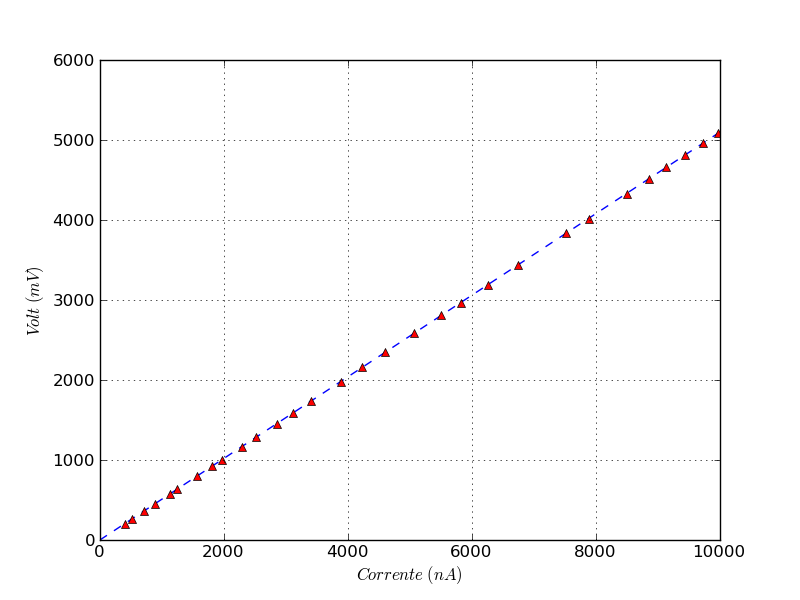
\includegraphics[scale=0.75]{grafici/C1/res1.png}
\
$\chi^2 = 5.76 $

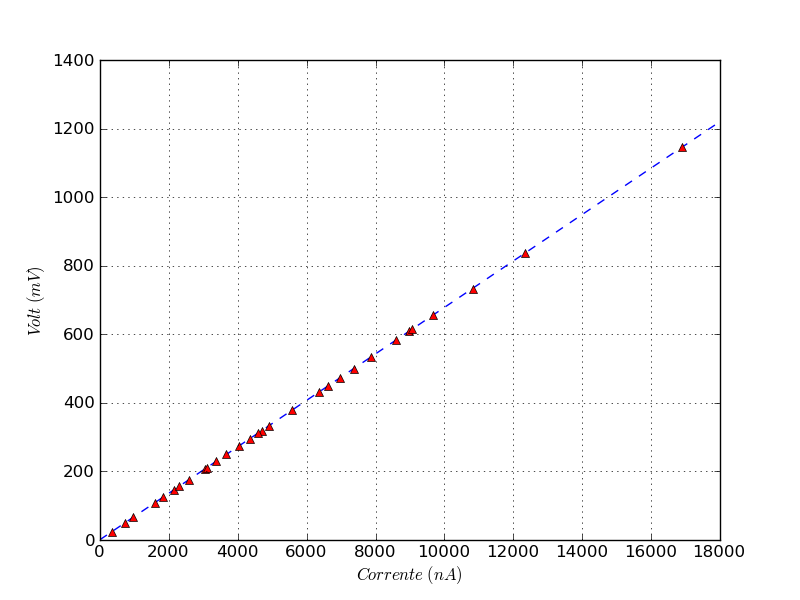
\includegraphics[scale=0.75]{grafici/C1/res2.png}

$\chi^2 = 4.88 $

Misuro la resistenza interna del voltometro, mantenendo costante la ddp a $14.5\ V$ e variando la resistenza all'interno del circuito. 
Il voltmetro è in parallelo al circuito, perciò $R_i$:

$$R_i = \frac{RV}{RI-V} $$

dove R è la resistenza variabile, I la corrente nel circuito e $V= 14.5\ V$

\begin{center}
\begin{tabular}{*{2}{c}}
Resistenza $M\Omega$ & Corrente $nA$\\
\midrule
7&      36\\
9&      32\\
10& 30\\
11&     29\\
12&     28\\
13&     27\\
14&     26\\
15&     26\\
16&     25\\
17&     24\\

\end{tabular}

La resistenza risulta $9.20 \pm 0.27 \ M \Omega$.


Misuriamo la resistenza interna dell'amperometro, che è collegato in serie al circuito. 

$$R_i = \frac{V-RI}{I}$$

In questo caso, R è fissato ($R=0.5 \Omega$) e sono V e I a variare
\begin{tabular}{*{2}{c}}
Volt $mV$ & Corrente $nA$\\
\midrule
22&      1769\\
40&      3271\\
60&      5047\\
105&     8938\\
133&     11201\\
142&     12021\\
164&     13882\\
174&     14745\\
208&     17604\\
232&     19671\\



\end{tabular}

La resistenza interna risulta $11.42 \pm 0.45 \Omega$


\end{center}


Colleghiamo una piccola lampada a filamento al circuito, e verifichiamo che il suo comportamento resistivo non segue la legge di Ohm. 

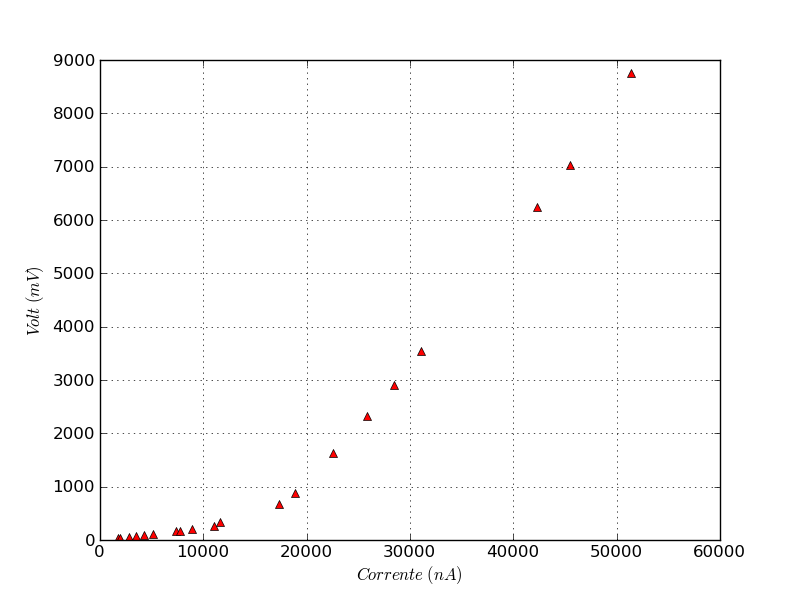
\includegraphics[scale=0.75]{grafici/C1/lampa.png}

La lampadina ha un comportamento non-ohmico nel momento in cui il filamento si scalda sufficientemente e inizia ad emettere luce ($500mV$).


\section{Partitore resistivo}

\subsection{Situazione senza carico}
\begin{center}
\begin{tabular}{*{2}{c}}
$V_{in}$ & $\frac{V_{in}}{V_{out}}$\\
\midrule
329.0 & 0.5015 \\
493.0 & 0.501 \\
544.0 & 0.5018 \\
618.0 & 0.5016 \\
667.0 & 0.5007 \\
776.0 & 0.5 \\
803.0 & 0.5006 \\
927.0 & 0.5005 \\
1078.0 & 0.5 \\
1285.0 & 0.4996 \\
\end{tabular}

\end{center}

$\chi^2=0.0169147373983$


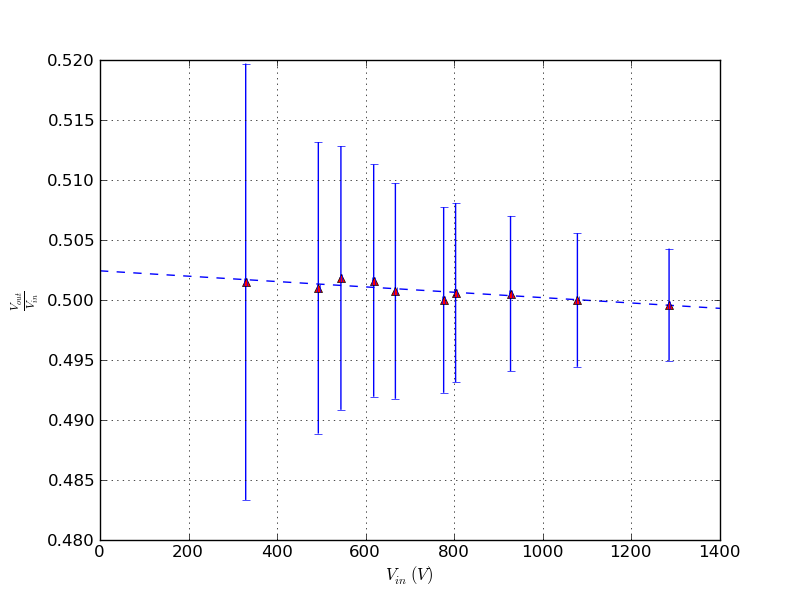
\includegraphics[scale=0.75]{grafici/C1/part1.png}

\subsection{Situazione con carico}
\begin{center}

\begin{tabular}{*{2}{c}}
$V_{in}$ & $\frac{V_{in}}{V_{out}}$\\
\midrule
220.0 & 3.1 \\
276.0 & 3.1051 \\
302.0 & 3.1126 \\
410.0 & 3.1073 \\
511.0 & 3.1115 \\
559.0 & 3.1055 \\
624.0 & 3.109 \\
752.0 & 3.109 \\
906.0 & 3.1093 \\
1036.0 & 3.111 \\
\end{tabular}

\end{center}
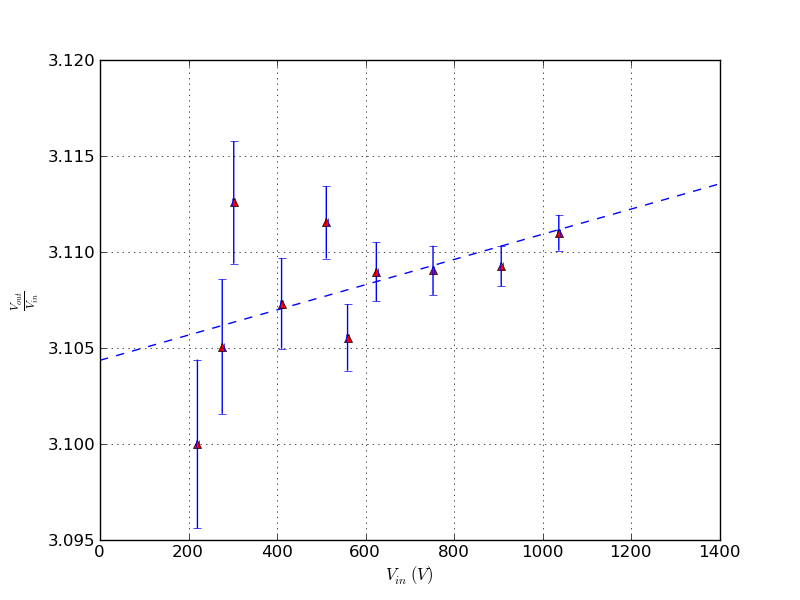
\includegraphics[scale=0.75]{grafici/C1/part2.png}

$\chi^2 = 12.9963702671$


\end{document} 



